\chapter{Analýza}
V tejto kapitole sa pozrieme na zopár problémov a ich riešení, na ktoré sme narazili počas vytvárania nášho analyzátoru.
Ako prvé sme sa museli rozhodnúť v akom jazyku budeme náš projekt implementovať. Na to si autor zvolil obecne rozšírený jazyk C++, pretože ho pozná najlepšie a má s ním najviac skúseností. Táto voľba nás zároveň v ničom zásadne neobmedzila a nemala negatívny dopad na celkový výsledok aplikácie. Teraz sa pozrieme na niekoľko konkrétnych problémov a spôsoby akými sme ich vyriešili.

\section{Získanie USB packetov}
Na získavanie USB paketov nám bude obecne slúžiť paket sniffer. Väčšina paket analyzátorov má implementované vlastné sniffery a preto sme sa o to pokúsili tiež. Narazili sme ale na niekoľko zásadných problémov, ktoré sa úzko viažu s platformou na ktorú cielime s našou aplikáciou~--~Windows.

Microsoft dokumentácia podrobnejšie opisuje komunikáciu medzi HID zaridením a kernel/user-mode aplikáciou~\cite{hid_opening_collections}. Pri tejto komunikácii sme schopní zachytiť USB pakety posielané zariadením a neskôr ich analyzovať. Keďže naša aplikácia beží v user-mode, prejdeme si práve tento spôsob komunikácie:
\begin{enumerate}
\item Aplikácia nájde a identifikuje HID zariadenie.
\item Aplikácia pomocou metódy \textit{CreateFile} otvorí spojenie s HID zariadením.
\item Aplikácia pomocou \textit{HID API}~\cite{hid_api} metód \textit{HidD\_Xxx} získa \textit{Preparsed Data} a informácie ohľadom HID zariadenia.
\item \label{kap03:read:paket} \textbf{Aplikácia použije metódu \textit{ReadFile} resp. \textit{WriteFile} na získanie inputu zariadenia resp. poslanie reportu zariadeniu.}
\item Aplikácia pomocou \textit{HID API}~\cite{hid_api} metód \textit{HidP\_Xxx} interpretuje HID reporty.
\end{enumerate}

Podstatný je práve bod~\ref{kap03:read:paket} v ktorom vidíme, že pomocou metódy \textit{ReadFile} sme schopní od daného zariadenia získať USB pakety, ktoré reprezentujú jeho input. Tie by sme následne mohli pomocou nášho analyzátoru spracovať. Tu narážame na prvý problém, ktorý sa priamo viaže na platformu Windows a ktorý si detailnejšie opíšeme v nasledujúcej sekcii.

\subsection{Windows exclusive mód}
Windows má definovaný tzv. \textit{Access Mode}, ktorý určuje restrikciu prístupu \textit{HID Clienta} k HID zariadeniu. 
Ten môže byť buď \textit{Shared} alebo \textit{Exclusive}. \textit{Exclusive Mode} zabraňuje ostatným \textit{HID Clientom} v zachytávaní alebo získavaní inputu HID zariadenia, pokiaľ nie sú hlavným príjemcom daného inputu. Preto z bezpečnostných dôvodov otvára \textit{RIM (Raw Input Manager)} niektoré zariadenia v \textit{Exclusive Mode}.

Ak je zariadenie otvorené v \textit{Exclusive Mode}, aplikácia má stále prístup k niektorým jeho údajom pomocou  \textit{HID API}~\cite{hid_api} metód  \textit{HidD\_\textbf{Get}Xxx}. Tieto metódy nám obecne umožnia získať niektoré descriptory zariadenia, tak ako aj jeho \textit{Preparsed Data}. Nie je nám ale umožnené volať metódu \textit{ReadFile}, takže nemáme akým spôsobom zachytávať komunikáciu HID zariadenia s clientom.

Tabuľka zariadení~\cite{hid_access} (obrázok~\ref{obr:kap3:access_mode}), ktoré \textit{RIM} otvára v \textit{Exclusive Mode} obsahuje aj tie, ktoré sme si v úvode zvolili ako podmnožinu HID zariadení na analýzu -- myš a klávesnica.

\begin{figure}[!htb]
	\centering
	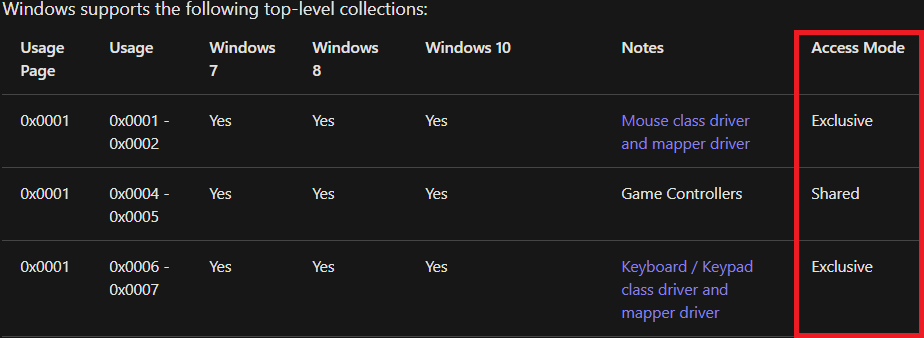
\includegraphics[width=\textwidth]{img/kap3_access_mode}
	\caption{Tabuľka zariadenía ich \textit{Access Mode}. Zariadenia postupne po riadkoch -- myš, joystick a klávesnica}
	\label{obr:kap3:access_mode}
\end{figure}

\subsection{Známe knižnice}
Keďže komunikáciu nemôžeme zachytávať priamo pomocou \textit{HID API}~\cite{hid_api} metód, rozhodli sme sa skúsiť použiť niektoré známe knižnice na sledovanie USB zbernice. 

Pravdepodobne najznámejšou z nich je \textit{libusb}~\cite{libusb} -- knižnica napísaná v jazyku C, ktorá slúži na poskytnutie prístupu k USB zariadeniu. Je cielená na programátorov aby im uľahčila vývoj aplikácií, ktoré komunikujú s USB hardwarom. Podporuje viaceré platformy, medzi ktorými sa nachádza aj Windows. Zároveň beží v user-mode, takže aplikácia ktorá ju využíva nepotrebuje žiadne špeciálne privilégiá na používanie libusb API. Ďalšou výhodou je, že podporuje všetky verzie USB od 1.0 až po 3.1. Je schopná zachytiť všetky typy prenosov (control,bulk,interrrupt,isochronus), a teda by sme pomocou nej mohli sledovať celú komunikáciu so zariadením vrátane počiatočného nakonfigurovania. Bohužiaľ, ani pomocou tejto knižnice sme neboli schopní získať prístup k zariadeniam, ktoré Windows otvára v exclusive móde.

Keďže sa zameriavame na HID zariadenia, skúsili sme hľadať niečo viac špecifické práve pre túto triedu USB zariadení, a to nás zaviedlo k \textit{HIDAPI}~\cite{hidapi_library}. \textit{HIDAPI} je ďalšia veľmi rozšírená knižnica, ktorá umožňuje komunikáciu s USB zariadeniami z HID triedy a takisto beží na viacerých patformách vrátane Windowsu. Pretrváva tu ale rovnaký problém ako s minulou knižnicou -- nie je možné získať prístup k zariadeniam, ktoré sú otvorené vo Windows exclusive móde.

Vyzerá to tak, že jediné riešenie nášho problému je priamo pracovať s filter driverom, ktorý sa nachádza na driver stacku daného zariadenia.

\subsection{Driver}
Windows ponúka niekoľko vstavaných driverov pre rôzne typy zariadení. Stačí ak nájdeme ten, ktorý nám umožní komunikáciu s konkrétnymi HID zariadeniami, s ktorými bol problém kvôli exclusive módu -- klávesnica a myš. Pre tieto dve konkrétne zariadenia momentálne existuje \textit{Moufiltr}~\cite{moufiltr} (upper-level filter driver pre myš) a \textit{Kbfiltr}~\cite{kbfiltr} (upper-level filter driver pre klávesnicu). Tie ale podporujú len legacy zariadenia -- non-USB, non-Bluetooth a non-I2C zariadenia.

Riešením by teda bolo naprogramovanie vlastného filter driveru pre myš a klávesnicu. Toto je ale už nad rámec našej práce a preto na získavanie USB paketov použijeme inú third-party aplikáciu.

\subsection{Third-party aplikácie}
Na zachytávanie USB paketov sme sa rozhodli použiť \textit{USBPcap}~\cite{usbpcap}, s ktorým sme sa už stretli v kapitole~\ref{uvod:sec:Wireshark} keď sme opisovali Wireshark a rôzne sniffery, s ktorými je schopný spolupracovať. USBPcap je veľmi rozšírený Windows sniffer USB paketov a jeho hlavnou výhodou je jednoduchá inštalácia. Takisto nám vyhovuje, že je s ním schopný spolupracovať Wireshark, čo nám častokrát počas vývoja poskytlo spôsob akým sme si mohli overiť správnosť nami vykonanej analýzy niektorých paketov. Daný sniffer zachytáva pakety do súborov v obecne známom formáte -- pcap~\cite{pcap}. 

Miernou nevýhodou je, že nepodporuje čítanie zo súboru do ktorého práve zapisuje -- analýzu paketov v reálnom čase tak budeme musieť vykonať trochu iným spôsobom, a to za pomoci Wiresharku. Ako sme už spomínali, Wireshark je schopný spolupráce s USBPcapom a zároveň podporuje ukladať výstup analýzy do súboru, ktorý je takisto formátu pcap. Wireshark už ale podporuje čítanie z daného súboru počas toho, ako do neho zapisuje. To znamená, že ak budeme chcieť vykonať analýzu v reálnom čase, urobíme to pomocou Wiresharku (konkrétnejší postup si ukážeme neskôr v užívateľskej dokumentácii v kapitole~\ref{udok:chap}).



\section{Sémantická reprezentácia dát}
Ako sme už naznačili v kapitole~\ref{uvod:sec:HID}, na vykonanie sémantickej analýzy inputu HID zariadenia je potrebné získať informácie o danom inpute z Report Descriptoru konkrétneho zariadenia. V tejto kapitole si vysvetlíme formát Report Descriptoru a ako nám informácie ktoré reprezentuje pomôžu v sémantickej analýze inputu HID zariadenia.


ako si z dat vytiahnut udaje ktore su potom pouzite na semanticku analyzu implementovanych HID zariadeni : HID Report parser, InputValues a EndpointDevice struct.
Nasledne sparovanie - ako vybrat spravny report pre konkretny input

\section{Spracovávanie pcap súborov}
moznosti ako citat pcap subory : bud pouzit uz existujucu kniznicu : na linuxe Libpcap, windows NPcap(deprecated WinPcap), alebo citat subory manualne : std::istream alebo QFile
\section{Voľba frameworku}
obecne co by som od toho GUI priblizne chcel, potom opisat preco som si vybral prave Qt a v nasledujucich kapitolach opisat rozhodnutia uz v Qt
dovod preco som si zvolil qt namiesto inych c++ GUI frameworkov(napriklad sfml)
\section{Zobrazenie základných informácií}
ako zobrazovat zakladne info o packete : pouzit QListWidget alebo QTableWidget (pripadne nieco ine ako nejaky abstract viewmodel), narok na zakladne funkcionality : lahka rozsiritenlnost o dalsie ''stlpceky'' , moznost jednoduchej interakcie(doubleClick na polozku). Mat vsetky info na jednom okne / mat pop-up okna. Farebne oddelenie.
\section{Zobrazenie sémantického významu dát}
ako vyzobrazit semanticky vyznam roznych dat - descriptory, usb header, vyznam input dat roznych HID zariadeni
\section{Hexdump}
ako v qt urobit hexdump - do coho zobrazovat data(vytvorit si vlastny viewer dedeny od QAbstractScrollArea, pripadne niecoho ineho) vs najst nieco co uz v qt je a upravit to aby to sedelo poziadavkam. Vziat do uvahy bezne funkcie hexdumpu : selection mody(oznacit naraz hexa a im odpovedajuce printable), logicke oddelenie dat(napriklad farbami)








